\documentclass{article}
	\usepackage{ctex}
    \usepackage{geometry}
        \geometry{left=2.54cm,right=2.54cm,top=2.54cm,bottom=2.54cm}
    \usepackage{graphicx}
    \usepackage{subfig}
    \begin{document}
	\title{信号与系统大作业 \\ [2ex] \begin{large} \emph{小白鲸找妈妈} \end{large} }
	\author{王晗\\(2013011076)}
	\date{\today}
	\maketitle
	\section{单频信号模拟}
		\subsection{whalesong.wav波形}
            \subsubsection*{读入whalesong.wav文件,听一听声音;绘制波形,解释波形和声音的关系}
            绘制波形如下图所示: 
            \begin{figure}[htb]
                \centering
                \subfloat[完整波形]
                {
                    \label{fig:origin-1}
                    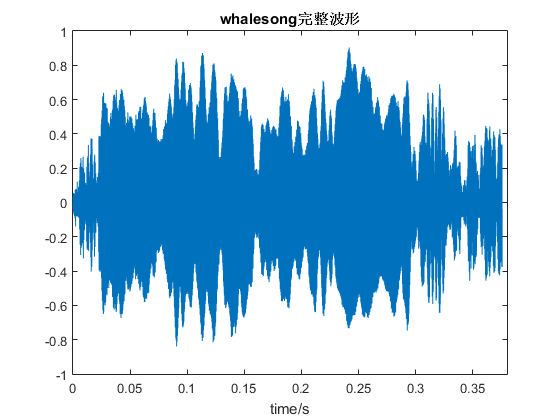
\includegraphics[width=7cm]{figure1.png}
                }
                \hspace{10pt}
                \subfloat[局部波形]
                {
                    \label{fig:origin-2}
                    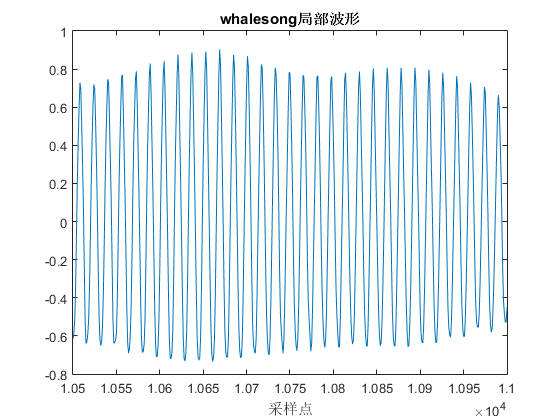
\includegraphics[width=7cm]{figure2.png}
                }
                \caption{whalesong波形}
                \label{fig:origin}
            \end{figure}
            
            将波形和实际的音频进行比较,可以发现波形振幅的表示声音的响度,波形的振动频率表示声音的频率。
            
            \subsubsection{如果要用一个单频信号模拟上述声音,请计算该信号的频率}
            

\end{document} 